
\chapter{\label{ch:problemformulatio}Problem Formulation and Radiosity Integral Equation}

In this section we formulate radiosity problem and derive corresponding radiosity integral equation. After defining the problem, possible solution methods, analytical and numerical, has been discussed at the end of the Chapter.


\section{\label{ch:problemformulation}Problem Definition}
The radiosity problem is special case of more general problem of global illumination. Radiosity is global illumination problem with scene composed of only lambertian (diffused) surfaces. Labertian surface are surface with lambertian reflectance i.e. apparent brightness of a point on the surface is equal from any view point above the surface. This is opposite to specular surface which are shiny surface. With this assumption of lambertian surfaces we now define the problem mathematically.

Radiosity $B(x_1,y_1)$ at point is power per unit area that leaves a point $(x_1,y_1)$ on a surface. The problem is to find the radiosity function  $B(x_1,y_1)$ over domain of all the surfaces in the scene given a following input,
\begin{itemize}
\item $E(x_1,y_1)$, radiosity of emitters(light source) of scene
\item $K(x_1,y_1,x_2,y_2)$, ratio of radiosity received by point $(x_1,y_1)$ to the radiosity of  point $(x_2,y_2)$\\
\item $p(x_1,y_1)$ reflectance of the surface at point $(x_1,y_1)$\\

\end{itemize}
Where, $(x_2,y_2)$,$(x_1,y_1)  \in  M^2$, two dimensional domain of all the surfaces in the  three dimensional scene $\in \mathbb{R}^3$.

$E(x_1,y_1)$ represents radiosity emitted by point $(x_1,y_1)$. It is non-zero for a light source and zero for other surfaces. $K(x_1,y_1,x_2,y_2)$ is calculated from geometry of the scene. The $K(x_1,y_1,x_2,y_2)$ is calculated from geometric location of the surfaces. For lambertian surface only one quantity,  $p(x_1,y_1)$, is required to describe reflectance.

For simplifying further discussion, we represent a point on surface by x. Kernel $K(x,y)$ can be expanded as shown in the eq. (\ref{eq:3dkernel}) which consist of cosine of angle made by local surface normals with a vector connecting two points, the distance  $r_{12}^{2}$ between the two points (see Figure \ref{xytheta}) and the visibility function which takes values from \{0,1\}, $0$ whene light ray can not travell from $y$ to $x$ due to an oclusion. The constant factor $\pi$ accounts for normalization of the integration. 

\begin{equation} \label{eq:3dkernel}
K(x,y) =  \frac{\cos \theta_x \cos \theta_y} {\pi r_{12}^{2}} V(x,y) \\ 
\end{equation}


\begin{figure}[h]
\centering
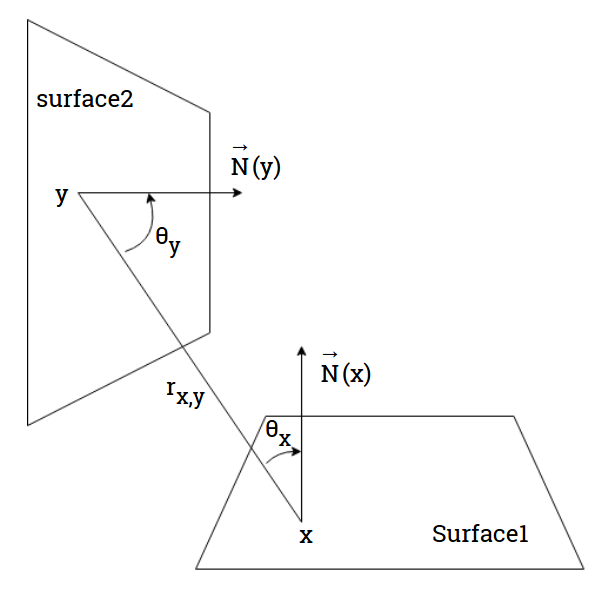
\includegraphics[width=0.4\linewidth]{xy.png}
\caption{Geometry in calculation of $K(x,y)$}
\label{fig:xytheta}
\end{figure}

\section {Radiosity Integral Equation}
Radiosity is governed by an non-homogeneous Fredholm integral equation of second kind (shown in Equation \ref{eq:NHFIEST}) which arises form more general problem of heat transfer known as rendering equation \cite{Kajiya} (see Appendix \ref{apen:derivationdegenerate}). In Equation \ref{eq:NHFIEST}, we solve integral equation for unknown function $\phi(x)$. 
\begin{equation} \label{eq:NHFIEST}
\phi(x)=f(x)+\lambda\int_{M^2} K(x,y)\phi(y)dy\quad x,y \in M^2
\end{equation}
In radosity, problem can be casted to integral equation shown in eq. (\ref{eq:genrie}). One way to relate equation with radiosity problem is that the radiosity $B(x)$ at point $(x)$  is sum of emitted radiosity $E(x)$ and reflected radiosity $p(x)K(x,y)B(y)$ which is received from all (integral) the points $y \in M^2$,  domain of all the surfaces in the scene.\\

\begin{equation} \label{eq:genrie}
B(x)=E(x)+p(x)\int_{M^2}K(x,y)B(y)dy
\end{equation}
In eq. (\ref{eq:genrie}) the integral is over all the points in domain of all  the surfaces $M^2$ in the scene. The kernel of integral equation is $p(x)K(x,y)$, which is calculated from geometry of input scene. Thus we can solve radiosity integral equation to solve radiosity problem.


% The parameters c and d takes value depending on  the scene. For 2D scenes, a scene consisting of lines instead of surfaces, d takes the value 1 and c takes the value 1/2 and the domain of the points is 1D. In the case of 3D scenes d takes the value 2 and c takes the value 1/$\pi$. From this point onwards we will refer to points by x and depending on the context (1D or  2D) it will be defined. The eq. (\ref{eq:3drie}) can be written as shown in eq. (\ref{eq:genrie})\\\\
% {\bf show equation (3)}
% \begin{equation} \label{eq:genrie}
% B(x)=E(x)+P(x)\int K(x,y)B(y)dy\\\\
% \end{equation}
\section{Analytical and Numerical Solution}
In literature lot of methods where developed to solve the non-homogeneous Fredholm integral of second kind \cite{iesurvey} \cite{ie}. In particular, if the kernel K is degenerate, one can find exact solution of the radiosity integral equation analytically \cite{ie}. But for even simple 2D  scene (flatland, see Chapetr \ref{ch:waveletprojection}), the kernel is non-degenerate. If analytical solution is not possible then one can solve the problem by approximation methods like Collocation Method, Galerkin Method \cite{iesurvey} \cite{ie}. We therefore use finite element methods(FEM) to compute approximate solution. We write unknown radiosity function as linear combination of basis function. Thus the problem get casted to system of linear equations which can be solved and approximate solution can be computed. In other words we solve the problem in finite dimensional function space instead of $L^2$ space, space of finite energy function. This method is also known as projection methods, more on these is discussed in next section.

